


\documentclass[pnumromarab,normaltoc]{abnt}			%Numera��o de acordo com UFPR

% Utilize a op��o normalfigtabnum para numerar as figuras e tabelas por cap�tulo

\usepackage[brazil]{babel}
\usepackage[latin1]{inputenc}
\usepackage{abnt-alf}
\usepackage{graphicx}														%Package para figuras

\makeatletter	%Para que ele entenda o @

% \documentclass{abnt}
% \usepackage[latin1]{inputenc}
% \usepackage[brazil]{babel}
% testando se os pacotes para uso com bibTeX são lidos
% \usepackage[num]{abntcite}

% \renewcommand{\folhadeaprovacao}{
% 
% }

\begin{document}
\autor{DIGITE SEU NOME}

\titulo{DIGITE O T�TULO}

\orientador{Nome do Orientador}

\comentario{Disserta��o apresentada como requisito parcial � obten��o do grau de bacharel em Ci�ncia da Computa��o, pelo Programa de Gradua��o, Setor, Universidade Federal do Pampa.}

\local{Alegrete}

\data{Junho 2010}


% ELEMENTOS PR�-TEXTUAIS
% Capa - Obrg
\capa
% Lombada
% Folha de rosto - Obrg
\folhaderosto
\addtocounter{page}{1} %Come�a a contar aqui :)
% Errata
% Folha de aprova��o - Obrg
\begin{titlepage}
\espaco{1.1}

\begin{center}
	\Large\textbf{{Termo de Aprova��o}}
\end{center}

\vspace{0.75cm}

\begin{center}
	\large\ABNTautordata
\end{center}

\vspace{1cm}

\begin{center}
	\large\ABNTtitulodata
\end{center}

\vspace{1cm}

\noindent Disserta��o aprovada como requisito parcial para obten��o do grau de Mestre/Doutor em Minha �rea, pelo Programa de P�s-Gradua��o, Setor, Universidade Federal do Paran�, pela seguinte banca examinadora:

\setlength{\ABNTsignthickness}{0.4pt}
\setlength{\ABNTsignskip}{2cm}

\vspace{-0.5cm}
\assinatura{Prof. Dr. Meu Orientador\\Universidade Federal do Paran�}

\vspace{-0.5cm}
\assinatura{Prof. Dr. Meu Co-orientador\\Universidade Federal do Paran�}

\vspace{-0.5cm}
\assinatura{Prof. Dr. Convidado\\Universidade}

\vspace{-0.5cm}
\assinatura{Prof. Dr. Convidado \\Universidade}

\vfill

\begin{center}
	Alegrete, xx de junho de 2010
\end{center}

\end{titlepage}
% Dedicat�ria(s)
\pretextualchapter{~}

\vfill
\hspace{.3\textwidth}
\begin{minipage}{.6\textwidth}
	\par $\phantom{linha em branco}$
 \begin{flushright}
    \par Dedico esse trabalho � minha amada esposa, Joseane, pela paci�ncia e apoio incondicional em todos meus projetos acad�micos e pessoais.
  \end{flushright}
  \par $\phantom{linha em branco}$
 \end{minipage}

\newpage

% ******** AGRADECIMENTOS *********
% *********** OPCIONAL ************
\pretextualchapter{Agradecimentos}

\hspace{.3\textwidth}
	\par Meu primeiro agradecimento vai para minha fam�lia, sem a qual eu n�o estaria aqui vivo. Agrade�o pela paci�ncia e pela compreens�o no momentos que mais precisei (principalmente nos v�rios meses sem visit�-los), pelas palavras de apoio e conforto (\emph{``logo logo termina!''}) e claro pela sua �ndole exemplar e conhecimento �nico que pude desfrutar durante minha vida. Muito obrigado por tudo, pai, m�e e mano, os aplausos s�o para voc�s tamb�m!
    \par Acho que eu n�o estaria aqui, escrevendo esse trabalho, se n�o fosse por meu querido mestre, tutor e amigo meu professor Vin�cius Jacques Garcia, ao qual eu deve grande parte de meu conhecimento, n�o s� acad�mico mas de exemplo de pessoa. Obrigado pelas conversas amigas e paci�ncia com minha
    \par Tamb�m deve dizer que sem uma outra pessoa eu n�o estaria aqui, que dizer, eu at� estaria mas possivelmente tomando algum tarja preta ou em uma consulta num psiquiatra, o que eu quero dizer � que se eu mantenho ainda um pouco de lucidez mental � gra�as a minha amada esposa Joseane (mas chamem-na de J�). Muito obrigado pelos �timos momentos ao seu lado, por ser minha companheira nas minhas id�ias geniais (leia-se loucas), pela for�a nas aulas de c�lculo e por rir das minhas piadas (pelo menos das boas).
    \par Agrade�o ao meu gato, que tem o nome de POG mas ningu�m chama ele pelo nome, por me fazer rir quando tentava pegar o cursor do mouse.
    \par Tenho um agradecimento especial aos professores que, juntamente com meu orientador me acompanharam, no decorrer da gradua��o compartilhando seu tempo, paci�ncia e conhecimento, contribuindo muito na minha forma��o. Obrigado Amanda, Vanessa, Diego, MC(Marcelo), Alessandro, Divane, Fabiane, Fernando, Daniel, Rog�rio, Ant�nio, Vin�cius(Montagner), Deise, Eduardo.
    \par Al�m do conhecimento na gradua��o levo tamb�m a amizade e companheirismo de de v�rios colegas do nosso curso e de outros tamb�m. Obrigado pelos momentos divertidos durante os trabalhos e momentos de estudo.
    \par \#finalDoTCC



% *********** EP�GRAFE ************
% *********** OPCIONAL ************
\pretextualchapter{~}

\vfill
\hspace{.3\textwidth}
\begin{minipage}{.6\textwidth}
	\par \emph{Voc� acha que o seu problema � s�rio? | exclamou Marvin, como se estivesse se dirigindo ao novo morador de uma sepultura | E eu? O que eu fa�o se eu sou um rob� man�aco-depressivo? N�o, nem tente me responder; eu sou 50 mil vezes mais inteligente que voc� e nem eu sei a resposta. S� de tentar me colocar no seu n�vel intelectual, fico com dor de cabe�a.}
	\par Douglas Adams | O Guia do Mochileiro das Galaxias
\end{minipage}
% Agradecimentos
% Ep�grafe
% Resumo em l�ngua vern�cula - Obrg
% Resumo em l�ngua estrangeira - Obrg
% Lista de ilustra��es
\listadefiguras
% Lista de tabelas
\listadetabelas
% Lista de abreviaturas e siglas
% Lista de s�mbolos
% Sum�rio - Obrg
\sumario
 
% ELEMENTOS TEXTUAIS
% Introdu��o Obrg
\chapter*{Introdu��o}
Em alguns setores de empresas, para efetuar o atendimento a um cliente, elas
devem deslocar um funcion�rio (ou uma equipe deles) da sua base de opera��es at�
a casa do cliente para executar o servi�o.
Isso ocorre principalmente em empresas que prestam algum tipo de servi�o de
atendimento domiciliar aos clientes, como por exemplo empresas de entrega de
correspond�ncia, provedores de internet no que diz respeito a suporte aos
clientes e companhias de distribui��o de energia el�trica tamb�m referente aos
suporte a clientes.
% Esse ultimo cen�rio que esse trabalho toma emprestado para os estudos de caso.

Esses tipos de atendimentos aos clientes s�o chamados de ordens de servi�o (OS)\sigla{OS} {Ordem de servi�o},
 podendo ter outros nomes conforme a �rea de atua��o da empresa, mas sempre com
 o intuito de registrar que a empresa deve fazer um atendimento a um determinado
cliente.
Cada OS contem alguns dados b�sicos como localiza��o do atendimento e tempo
previsto de atendimento. Trataremos aqui a localiza��o como um ponto no espa�o
$\Re^{2}$ e o tempo como a demanda de tempo que a OS levar� para ser atendida.

Como medida de deslocamento apenas consideraremos apenas a dist�ncia euclidiana
entre os pontos, pois algumas inst�ncias reais se fossem representadas com a
dist�ncia real que a equipe percorreria, iria demandar um mapa completo da
localidade e m�os das ruas, o que nem sempre � dispon�vel.

Nesse cen�rio de estudo tomamos algumas premissas como v�lidas:
\begin{itemize}
 \item Uma OS deve ser atendida por um funcion�rio/equipe;
 \item N�o levamos em considera��o agendamentos de hor�rios, apenas que todas as OS devem ser executas;
 \item Uma OS possui um tempo que a equipe levar� para exuta-la;
 \item Uma equipe consegue executar todas as OS atribuidas a ela no tempo estimado e predefinido de cada uma delas;
 \item O tempo de atendimento de todas as ordens atribuidas a uma equipe n�o deve ultrapassarem sua jornada de trabalho que � pr�viamente estipulada;
 \item As ordens s�o as de apenas um dia. As que entrarem durante o atendimento ficam agendadas o pr�ximo dia.
 \item N�o ser� considerado o tempo de deslocamento entre os atendimentos das OS.
\end{itemize}

Essas premissas definem o PDOS \sigla{PDOS} {Problema de Despacho de Ordens de Servi�o}, onde
devemos associar todas OS as equipes de modo que uma OS seja atendida por uma, e n�o mais que uma, equipe.
Minimizar o deslocamento entre os atendimentos � algo desej�vel para as empresas, pois diminui os custos e o tempo de deslocamento entre os atendimentos pela menor dist�ncia percorrida.

Ao designar um conjunto de OS a uma equipe, deve-se levar em considera��o a  carga hor�ria de cada mesma e a demanda de tempo que cada OS do conjunto.
 Isso por si s� pode ser visto como um Problema da Mochila, o que j� n�o � um problema de solu��o trivial.

Ao atribuir as OS levando em considera��o apenas a carga hor�ria da equipe e o tempo demandado pelas OS pode nos levar a solu��es como as apresentadas na figura \ref{FigDemandaCapacidade}, onde temos 3 equipes atendendo um total de 15 atendimentos.
\begin{figure}
 \begin{center}
  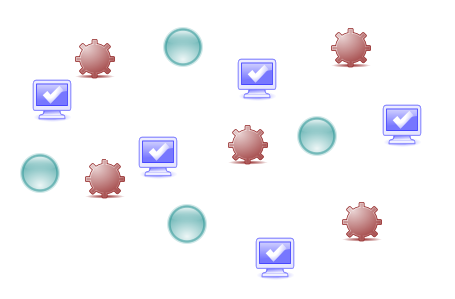
\includegraphics[scale=0.5]{./images/DemandasCapacidade.png}
 % DemandasCapacidade.png: 455x299 pixel, 96dpi, 12.04x7.91 cm, bb=0 0 341 224
  \end{center}
\caption{\label{FigDemandaCapacidade}Aloca��o de OS apenas pelas Demandas e
Capacidades }
\end{figure}

� poss�vel perceber que os atendimentos de cada equipe encontram-se
dispersos, necessitando um maior deslcomento das equipes de um atendimento a
outro do que se os atendimentos estivessem agrupados mais pr�ximos.

Um problema que engloba essas caracter�sticas apresentadas � o  CCP \sigla{CCP} {Problema de Agrupamento Capacitado - Capacitated Clustering Problem}, cl�ssico na literatura e tamb�m conhecido como (CPMP) \sigla {CPMP}{Problema das P-Medianas Capacitado - Capacitated P-Medians Problem}.
 Na figura \ref{FigCCPIntro} temos um exemplo de como as ordens de servi�o poderiam estar associadas �s equipes.

� poss�vel perceber que ainda assim n�o foi poss�vel atribuir as OS de modo que todas OS de de uma equipe fique pr�ximas de uma OS escolhida como centro.
 Isso � devido as restri��es de capacidade das equipes e demandas das OS.

\begin{figure}
 \begin{center}
  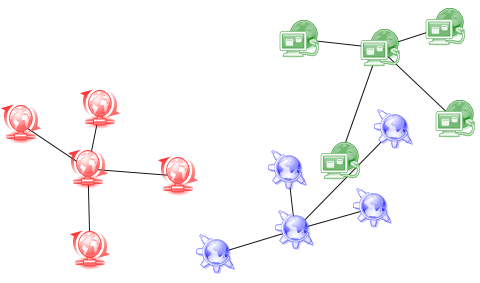
\includegraphics[scale=0.5]{./images/CCPIntro.png}
 % DemandasCapacidade.png: 455x299 pixel, 96dpi, 12.04x7.91 cm, bb=0 0 341 224
  \end{center}
\caption{\label{FigCCPIntro} Poss�vel atribui��o das Mesmas OS segundo CCP }
\end{figure}

As inst�ncias in�ditas desse problema foram retiradas de ordens de atendimento
de um concession�ria de distribui��o de energia el�trica e tiveram que ter a
capacidade de atendimento normalisadas para ser poss�vel gerar solu��es v�lidas
do problema. Esse fato ocorre pelo fato de encontrar uma solu��o � necess�rio
existir uma folga entre das demandas e a capacidade. � frente neste trabalho ser�
apresentado um estudo sobre essas folgas.

Nesse trabalho n�o trataremos da gera��o de rotas entre os atendimentos, mas
esse problema j� foi tratado na literatura como o CTSP \sigla{CTSP} {Problema do Caixeiro Viajante
Agrupado - Clustered Travel Salesman Problem}, onde desejamos entrar os menor ciclo Hamiltoniano nos pontos, sendo que os pontos
dos agrupamentos devem ser visitados em sequ�ncia \cite{jeanCTSP-Genetic}.

 %Inclui arquivo introducao.tex
% Desenvolvimento - Obrg
\chapter{Revis�o Bibliogr�fica}

\chapter{Segundo Cap�tulo}

\chapter{Terceiro Cap�tulo}
segundo esse cara \cite {RePEc:eee:ejores:v:18:y:1984:i:3:p:339-348} Tofu! 
% Conclus�o - Obrg
\chapter*{Considera��es Finais}

% Neste trabalho apresentamos a aplica��o de heur�sticas e m�todos de otimiza��o para o problema de agrupamento capacitado. O problema de agrupamento capacitado � um problema que representa em parte o problema de despacho de ordens de servi�o, por isso ele foi estudado nesse trabalho, sendo o PDOS o nosso cen�rio de aplica��o. 

Apresentamos aqui neste trabalho uma vis�o do PDOS como um CCP, fazendo uso de m�todos j� existentes em um problema relativamente novo. Dos m�todos tratados, procuramos abordar os m�todos heur�sticos mais tratados da literatura e compara-los quando aplicados aos dados do PDOS.

Dentre os m�todos trabalhados, os que apresentaram melhores solu��es foram o Random density e o Density, sendo o primeiro uma varia��o do segundo, com a diferen�a de inserir elementos de aleatoriedade para escolha dos centros, n�o desconsiderando o c�lculo de densidade o qual nos d� um bom indicativo de onde devem ser inseridos os centros. Mas, apesar de os valores obtidos serem menores que os demais m�todos, o seu tempo de computa��o � cerca de 3 vezes mais alto que o levado pelo m�todo density, que para inst�ncias com grande n�mero de indiv�duos e de centros (por exemplo algumas inst�ncias com mais de 3.000 pontos e 600 agrupamentos), tem um tempo de computa��o bastante alto. Esse tempo elevado n�o desqualifica o uso do m�todo para essa classe de problemas, visto que os atendimentos s�o processados por cidades como apresentado nas inst�ncias AE e possuem grande n�mero de atendimentos e poucas equipes.

Dos demais m�todos, Farthest � uma heur�stica construtiva que gera solu��es de baixa qualidade mas rapidamente. HMeans gera solu��es de qualidade boas de modo at� mais r�pida que o �ltimo. JMeans gera solu��es de qualidade boa tamb�m, mas com a desvantagem de ser extremamente lento na fase de busca de novos centros e reassocia��o dos indiv�duos. Essa etapa dessa heur�stica pode sofrer melhorias para acelerar como um todo o algoritmo, visto que essa � a etapa mais repetida durante as itera��es. Como exemplo de melhoria seria a diminui��o do n�mero de centros removidos para a inser��o de um novo centro para apenas os centros mais pr�ximos a esse novo centro, evitando que se insira um centro onde j� exista um grande n�mero de centros.

As ferramentas computacionais tamb�m ficam como contribui��o para futuros trabalhos ou de base para implementa��o de novos algoritmos fornecendo toda representa��o do problema bem como a visualiza��o do mesmo para an�lise dos dados.

Para trabalhos futuros consideramos a utiliza��o de m�todos h�bridos, onde m�todos exatos seriam utilizados apenas para resolver subproblemas de complexidade menor e utiliza��o de buscas locais com espa�o de busca ampliado pela relaxa��o de algumas restri��es, gerando solu��es infact�veis mas com valor da fun��o objetivo melhor que serviria de base para uma nova busca por solu��es fact�veis em uma vizinhan�a que anteriormente n�o era alcan��vel ou que exigia grande refinamento na etapa de busca local. Outra considera��o a ser levada para os trabalhos futuros � que para aplica��es em cen�rios reais, deve-se levar em considera��o o deslocamento entre ordens de servi�o, o que iria contribuir para o aumento do tempo (valor da demanda) para a equipe que est� atendendo as ordens de servi�o e  a carga hor�ria das equipes poder ser vari�vel de uma para outra. Nesse caso ter�amos um problema heterog�neo quanto a capacidade e tamb�m ter�amos o problema de roteiriza��o das OS, sendo que ao calcular uma rota pode acontecer de aumentar tempo, devido a um maior deslocamento entre os novos atendimentos, para um valor al�m da capacidade da equipe, gerando uma solu��o infact�vel.

A parte construtiva das heur�sticas tamb�m permitem trabalhos futuros no que diz respeito a escolha de indiv�duos como centros iniciais. A escolha com o c�lculo por densidade se mostrou muito boa, mas se forem utilizados dados estat�sticos � poss�vel de se definir os centros com melhores caracter�scas. Para isso seria necess�rio a aplica��o de algum m�todo como o GRASP \cite{feo1989probabilistic} onde uma solu��o fornece dados para a gera��o de uma nova solu��o.
 %Inclui arquivo conclusao.tex

% ELEMENTOS P�S-TEXTUAIS
% Refer�ncias - Obrg
\bibliography{../bibitex/bibliography_CCP} %Seu arquivo Bibitex

% Gloss�rio
% Ap�ndice(s)

% Anexo(s)
% \appendix

% \part*{Anexos}


% \chapter*{Anexo A: Diagramas UML}
% \renewcommand{\thefigure}{A.\arabic{figure}}
%
% \begin{figure}[ht]
%  \centering
%  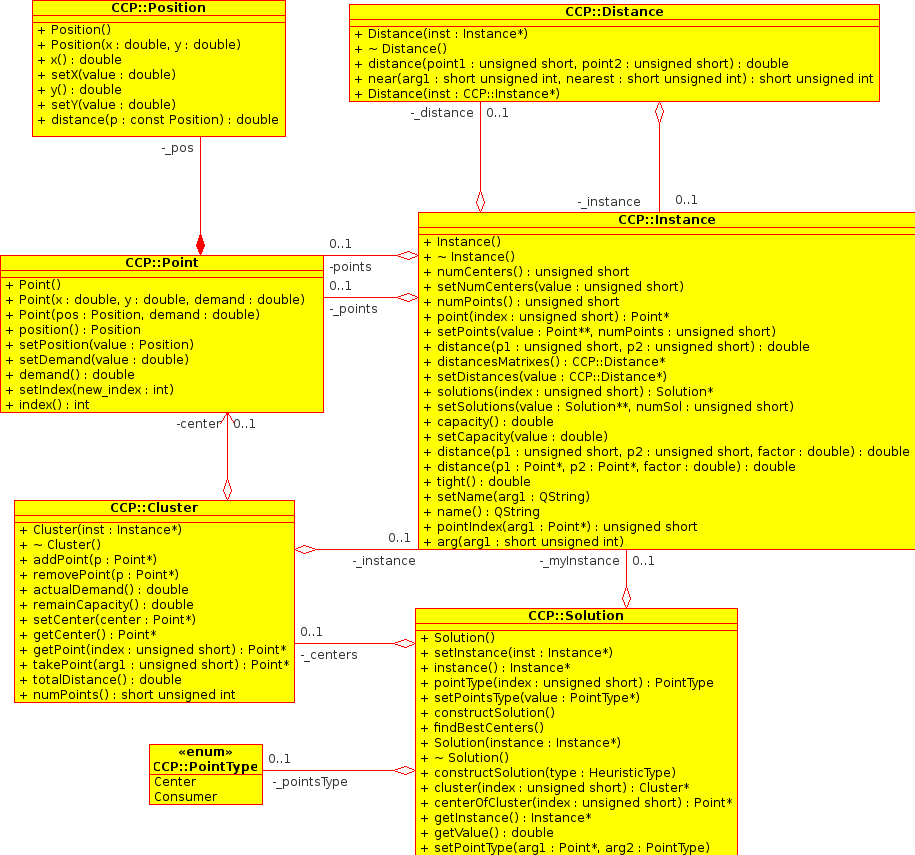
\includegraphics[bb=0 0 794 742,scale=0.4]{../TCC-I/imagens/Instance.png}
%  % Instance.png: 915x855 pixel, 83dpi, 28.00x26.16 cm, bb=0 0 794 742
% \caption{Classes que representam uma Inst�ncia e as solu��es }
% \end{figure}
%
% %
% % \begin{figure}
% %  \begin{center}
% %  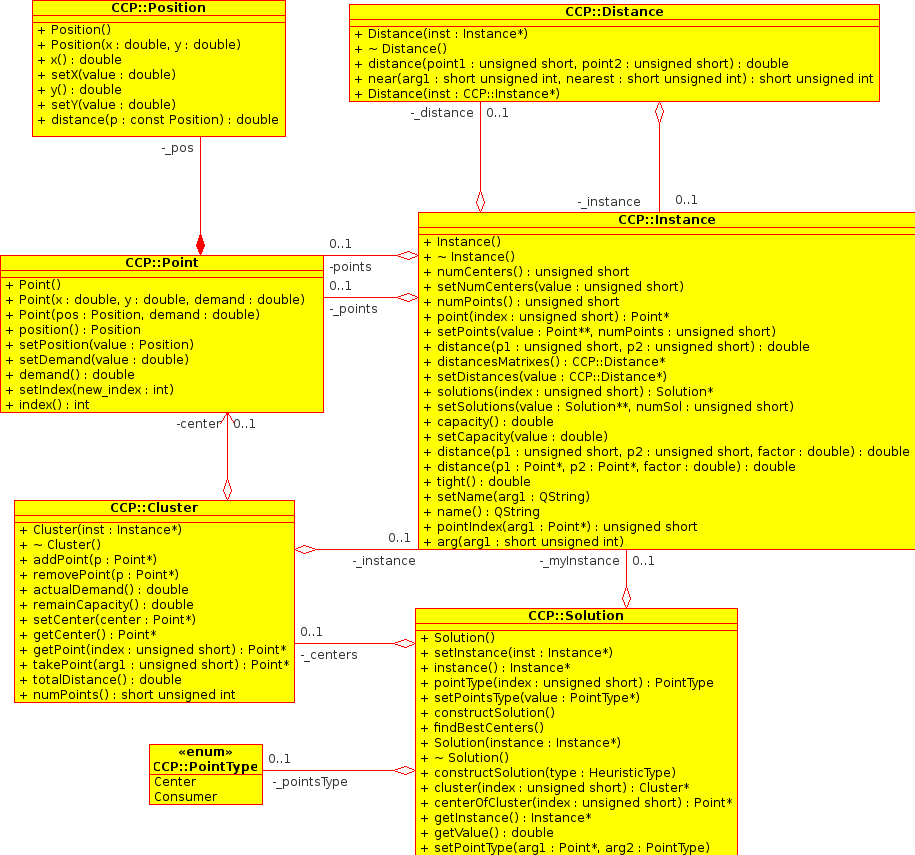
\includegraphics[scale=0.4]{../TCC-I/imagens/Instance.png}
% %  % Instance.png: 915x855 pixel, 83dpi, 28.00x26.16 cm, bb=0 0 794 742
% %
% % \end{center}
% % \end{figure}
%
%
% \begin{figure}[ht]
%  \centering
%  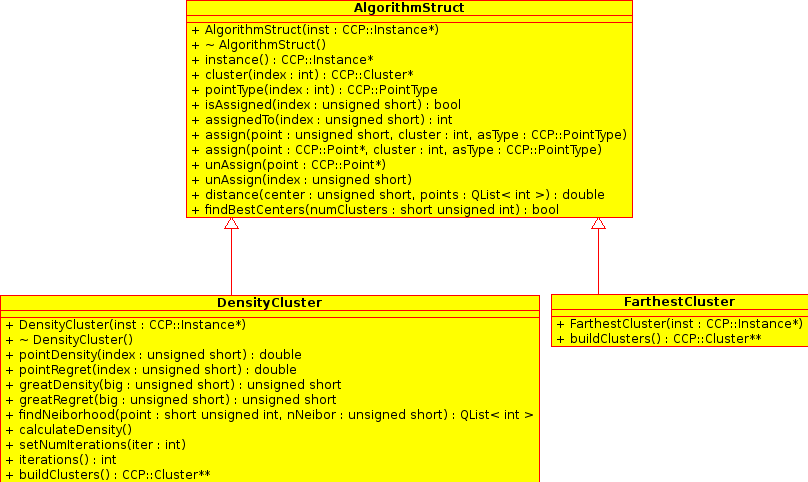
\includegraphics[bb=0 0 701 418, scale=0.6]{../TCC-I/imagens/Algorthms.png}
%  % Algorthms.png: 808x482 pixel, 83dpi, 24.72x14.75 cm, bb=0 0 701 418
% \caption{Classes dos algoritmos das heur�sticas de constru��o}
%
% \end{figure}
% %
% % \begin{figure}
% % \begin{center}
% % 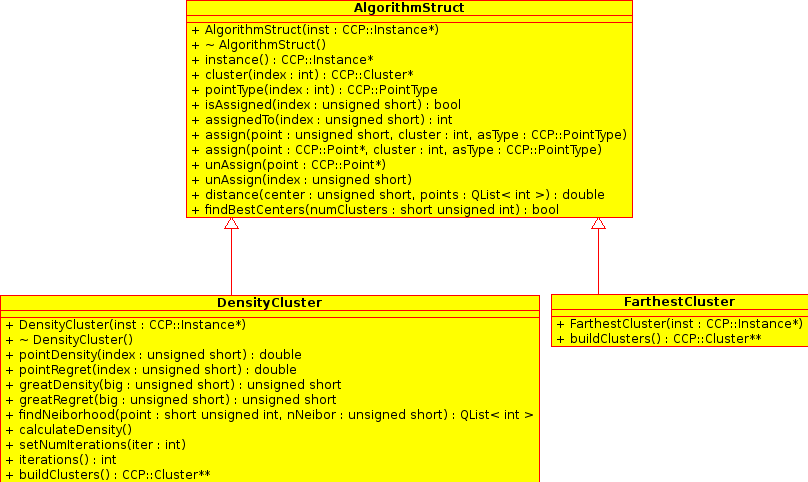
\includegraphics[scale=0.5]{../TCC-I/imagens/Algorthms.png}
% %
% % \end{center}
% % \end{figure}
%
%
% % \begin{landscape}
%
%
% \chapter*{Anexo B: Associa��o dos M�dulos}
% \renewcommand{\thefigure}{B.\arabic{figure}}
% %
% % 
\tikzset{
  arrow/.style={-stealth', line width=0.5pt},
  every picture/.append style={line width=1pt},
}

\tiny {

\enlargethispage{100cm}
% Start of code
% \begin{tikzpicture}[anchor=mid,>=latex',join=bevel,]
\begin{tikzpicture}[>=latex',join=bevel,scale=0.65]
  \pgfsetlinewidth{1bp}
%%
\pgfsetcolor{black}
  % Edge: node0 -> node4
  \draw [->] (130.06bp,219.43bp) .. controls (125.48bp,210.75bp) and (119.51bp,199.45bp)  .. (109.32bp,180.13bp);
  % Edge: node9 -> node12
  \draw [->] (716.02bp,147.39bp) .. controls (712.23bp,146.19bp) and (708.43bp,145.04bp)  .. (704.75bp,144bp) .. controls (632.92bp,123.76bp) and (612.69bp,127.83bp)  .. (540.75bp,108bp) .. controls (537.36bp,107.07bp) and (533.87bp,106.04bp)  .. (520.57bp,101.88bp);
  % Edge: node0 -> node11
  \draw [->] (108.83bp,226.23bp) .. controls (86.415bp,218.52bp) and (56.87bp,204.27bp)  .. (42.75bp,180bp) .. controls (31.694bp,161bp) and (36.774bp,136.1bp)  .. (47.572bp,107.83bp);
  % Edge: node6 -> node1
  \draw [->] (392.12bp,147.43bp) .. controls (390.6bp,139.01bp) and (388.64bp,128.14bp)  .. (385.02bp,108.13bp);
  % Edge: node9 -> node3
  \draw [->] (730.64bp,147.43bp) .. controls (710.16bp,136bp) and (681.55bp,120.03bp)  .. (650.79bp,102.86bp);
  % Edge: node8 -> node2
  \draw [->] (661.03bp,147.43bp) .. controls (677.35bp,137.64bp) and (699.21bp,124.52bp)  .. (726.54bp,108.13bp);
  % Edge: node5 -> node1
  \draw [->] (288.43bp,147.43bp) .. controls (304.26bp,137.68bp) and (325.46bp,124.64bp)  .. (352.29bp,108.13bp);
  % Edge: node2 -> node10
  \draw [->] (723.61bp,74.684bp) .. controls (720.65bp,73.658bp) and (717.67bp,72.741bp)  .. (714.75bp,72bp) .. controls (615.37bp,46.802bp) and (311.96bp,27.968bp)  .. (174.49bp,20.41bp);
  % Edge: node0 -> node1
  \draw [->] (143.2bp,219.19bp) .. controls (151.34bp,199.15bp) and (168.56bp,163.65bp)  .. (194.75bp,144bp) .. controls (234.16bp,114.43bp) and (289.34bp,101.03bp)  .. (339.68bp,93.545bp);
  % Edge: node5 -> node12
  \draw [->] (310.78bp,147.35bp) .. controls (344.57bp,136.56bp) and (391.55bp,121.49bp)  .. (432.75bp,108bp) .. controls (435.9bp,106.97bp) and (439.14bp,105.9bp)  .. (452.2bp,101.58bp);
  % Edge: node9 -> node2
  \draw [->] (756.75bp,147.43bp) .. controls (756.75bp,139.1bp) and (756.75bp,128.37bp)  .. (756.75bp,108.13bp);
  % Edge: node4 -> node1
  \draw [->] (147.76bp,147.85bp) .. controls (152.48bp,146.52bp) and (157.2bp,145.22bp)  .. (161.75bp,144bp) .. controls (218.97bp,128.68bp) and (285.01bp,112.7bp)  .. (339.44bp,99.83bp);
  % Edge: node8 -> node3
  \draw [->] (634.93bp,147.43bp) .. controls (633.86bp,138.89bp) and (632.48bp,127.82bp)  .. (629.95bp,107.6bp);
  % Edge: node6 -> node12
  \draw [->] (413.37bp,147.43bp) .. controls (426.18bp,137.4bp) and (443.46bp,123.88bp)  .. (466.24bp,106.05bp);
  % Edge: node7 -> node3
  \draw [->] (535.22bp,147.43bp) .. controls (553.25bp,136.24bp) and (578.27bp,120.71bp)  .. (606.27bp,103.33bp);
  % Edge: node6 -> node3
  \draw [->] (441.9bp,147.43bp) .. controls (483.67bp,134.52bp) and (544.13bp,115.84bp)  .. (594.23bp,100.36bp);
  % Edge: node4 -> node10
  \draw [->] (103.3bp,143.76bp) .. controls (108.09bp,119.09bp) and (116.69bp,74.86bp)  .. (124.23bp,36.09bp);
  % Edge: node0 -> node2
  \draw [->] (166.67bp,232.82bp) .. controls (294.44bp,227.45bp) and (803bp,204.6bp)  .. (825.75bp,180bp) .. controls (845.2bp,158.96bp) and (820.23bp,132.75bp)  .. (786.59bp,108.02bp);
  % Edge: node5 -> node3
  \draw [->] (320.06bp,147.35bp) .. controls (325.01bp,146.17bp) and (329.97bp,145.03bp)  .. (334.75bp,144bp) .. controls (425.61bp,124.41bp) and (449.45bp,125.42bp)  .. (540.75bp,108bp) .. controls (552.59bp,105.74bp) and (565.3bp,103.19bp)  .. (587.08bp,98.686bp);
  % Edge: node9 -> node1
  \draw [->] (717.25bp,147.4bp) .. controls (713.06bp,146.14bp) and (708.84bp,144.97bp)  .. (704.75bp,144bp) .. controls (589.21bp,116.65bp) and (553.22bp,135.4bp)  .. (423.85bp,105.62bp);
  % Edge: node7 -> node2
  \draw [->] (557.1bp,147.39bp) .. controls (561.03bp,146.21bp) and (564.95bp,145.07bp)  .. (568.75bp,144bp) .. controls (630.08bp,126.78bp) and (649.56bp,128.97bp)  .. (723.47bp,104.84bp);
  % Edge: node7 -> node12
  \draw [->] (506.69bp,147.43bp) .. controls (503.72bp,138.86bp) and (499.86bp,127.75bp)  .. (492.95bp,107.86bp);
  % Edge: node4 -> node11
  \draw [->] (88.899bp,143.83bp) .. controls (83.973bp,135.58bp) and (78.049bp,125.66bp)  .. (67.448bp,107.91bp);
  % Edge: node0 -> node3
  \draw [->] (166.8bp,232.75bp) .. controls (292.79bp,227.2bp) and (786.63bp,203.97bp)  .. (808.75bp,180bp) .. controls (819.6bp,168.24bp) and (818.31bp,156.83bp)  .. (808.75bp,144bp) .. controls (800.64bp,133.12bp) and (727.4bp,113.75bp)  .. (666.77bp,99.032bp);
  % Edge: node8 -> node1
  \draw [->] (581.63bp,147.41bp) .. controls (530.71bp,133.94bp) and (459.89bp,115.19bp)  .. (423.96bp,105.19bp);
  % Edge: node8 -> node12
  \draw [->] (606.39bp,147.43bp) .. controls (582.94bp,136.17bp) and (550.32bp,120.52bp)  .. (515.79bp,103.94bp);
  % Edge: node0 -> node10
  \draw [->] (108.77bp,225.48bp) .. controls (85.409bp,217.26bp) and (53.194bp,202.69bp)  .. (32.75bp,180bp) .. controls (9.7676bp,154.49bp) and (11.08bp,141.75bp)  .. (4.7496bp,108bp) .. controls (1.7995bp,92.274bp) and (-3.9994bp,85.396bp)  .. (4.7496bp,72bp) .. controls (20.241bp,48.28bp) and (48.728bp,34.912bp)  .. (84.051bp,24.816bp);
  % Edge: node7 -> node1
  \draw [->] (485.44bp,147.43bp) .. controls (467.6bp,137.55bp) and (443.66bp,124.29bp)  .. (414.48bp,108.13bp);
  % Node: node11
\begin{scope}
  \definecolor{strokecol}{rgb}{0.0,0.0,0.0};
  \pgfsetstrokecolor{strokecol}
  \draw (57bp,90bp) ellipse (43bp and 18bp);
  \draw (56.75bp,90bp) node {libQtGui.so};
\end{scope}
  % Node: node10
\begin{scope}
  \definecolor{strokecol}{rgb}{0.0,0.0,0.0};
  \pgfsetstrokecolor{strokecol}
  \draw (128bp,18bp) ellipse (47bp and 18bp);
  \draw (127.75bp,18bp) node {libQtCore.so};
\end{scope}
  % Node: node12
\begin{scope}
  \definecolor{strokecol}{rgb}{0.0,0.0,0.0};
  \pgfsetstrokecolor{strokecol}
  \draw (487bp,90bp) ellipse (45bp and 18bp);
  \draw (486.75bp,90bp) node {libQtTest.so};
\end{scope}
  % Node: node9
\begin{scope}
  \definecolor{strokecol}{rgb}{0.0,0.0,0.0};
  \pgfsetstrokecolor{strokecol}
  \draw (800bp,168bp) -- (757bp,180bp) -- (714bp,168bp) -- (714bp,147bp) -- (800bp,147bp) -- cycle;
  \draw (756.75bp,162bp) node {CCPTest};
\end{scope}
  % Node: node8
\begin{scope}
  \definecolor{strokecol}{rgb}{0.0,0.0,0.0};
  \pgfsetstrokecolor{strokecol}
  \draw (696bp,168bp) -- (637bp,180bp) -- (578bp,168bp) -- (578bp,147bp) -- (696bp,147bp) -- cycle;
  \draw (636.75bp,162bp) node {CCPSolution};
\end{scope}
  % Node: node1
\begin{scope}
  \definecolor{strokecol}{rgb}{0.0,0.0,0.0};
  \pgfsetstrokecolor{strokecol}
  \draw (424bp,108bp) -- (340bp,108bp) -- (340bp,72bp) -- (424bp,72bp) -- cycle;
  \draw (381.75bp,90bp) node {CCPModelLib};
\end{scope}
  % Node: node0
\begin{scope}
  \definecolor{strokecol}{rgb}{0.0,0.0,0.0};
  \pgfsetstrokecolor{strokecol}
  \draw (167bp,240bp) -- (138bp,252bp) -- (109bp,240bp) -- (109bp,219bp) -- (167bp,219bp) -- cycle;
  \draw (137.75bp,234bp) node {CCP};
\end{scope}
  % Node: node3
\begin{scope}
  \definecolor{strokecol}{rgb}{0.0,0.0,0.0};
  \pgfsetstrokecolor{strokecol}
  \draw (628bp,108bp) -- (550bp,90bp) -- (628bp,72bp) -- (706bp,90bp) -- cycle;
  \draw (627.75bp,90bp) node {CCPAlgorithms};
\end{scope}
  % Node: node2
\begin{scope}
  \definecolor{strokecol}{rgb}{0.0,0.0,0.0};
  \pgfsetstrokecolor{strokecol}
  \draw (790bp,108bp) -- (724bp,108bp) -- (724bp,72bp) -- (790bp,72bp) -- cycle;
  \draw (756.75bp,90bp) node {CCPIOLib};
\end{scope}
  % Node: node5
\begin{scope}
  \definecolor{strokecol}{rgb}{0.0,0.0,0.0};
  \pgfsetstrokecolor{strokecol}
  \draw (326bp,168bp) -- (265bp,180bp) -- (204bp,168bp) -- (204bp,147bp) -- (326bp,147bp) -- cycle;
  \draw (264.75bp,162bp) node {CCPDistance};
\end{scope}
  % Node: node4
\begin{scope}
  \definecolor{strokecol}{rgb}{0.0,0.0,0.0};
  \pgfsetstrokecolor{strokecol}
  \draw (148bp,180bp) -- (52bp,180bp) -- (52bp,144bp) -- (148bp,144bp) -- cycle;
  \draw (99.75bp,162bp) node {CCPClusterView};
\end{scope}
  % Node: node7
\begin{scope}
  \definecolor{strokecol}{rgb}{0.0,0.0,0.0};
  \pgfsetstrokecolor{strokecol}
  \draw (560bp,168bp) -- (512bp,180bp) -- (464bp,168bp) -- (464bp,147bp) -- (560bp,147bp) -- cycle;
  \draw (511.75bp,162bp) node {CCPRead};
\end{scope}
  % Node: node6
\begin{scope}
  \definecolor{strokecol}{rgb}{0.0,0.0,0.0};
  \pgfsetstrokecolor{strokecol}
  \draw (446bp,168bp) -- (395bp,180bp) -- (344bp,168bp) -- (344bp,147bp) -- (446bp,147bp) -- cycle;
  \draw (394.75bp,162bp) node {CCPModel};
\end{scope}
%
\end{tikzpicture}
% End of code

}
% \begin{figure}[ht]
%  \centering
%  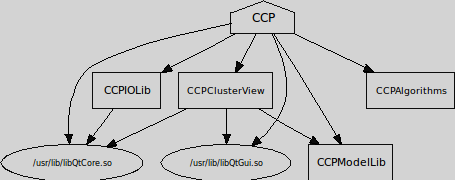
\includegraphics[bb=0 0 341 135]{./images/Modules.png}
%  % Modules.png: 455x180 pixel, 96dpi, 12.04x4.76 cm, bb=0 0 341 135
%
% \caption{Bibliotecas que fazem parte do sistema.}
%
% \end{figure}


% \end{landscape}



\end{document}



